%%%%%%%%%%%%%%%%%%%
% SECTION: CNN
%%%%%%%%%%%%%%%%%%%
\section{Convolutional Neural Networks}
Convolutional Neural Networks (CNN) is a special kind of ANN. The modern version of a CNN was first introduced by LeCun and Bottou \cite{LeCun1998Gradient-basedRecognition} in 1998. The authors claim that CNNs are inspired by how mammals visually perceive the world using architecture of neurons. Their work was inspired by a research investigation by Hubel and Wiesel \cite{Hubel1968ReceptiveCortex.} in which they describe in detail the mammal's visual perception architecture. Both LeCun and Bottou proposed a CNN called LeNet 5. This new model established a new state of the art in computer vision using a well known dataset for hand-written digits and words, the MNIST \cite{LeCun2010MNISTDatabase} dataset.

% FIGURE: lenet
\begin{figure}[!htb]	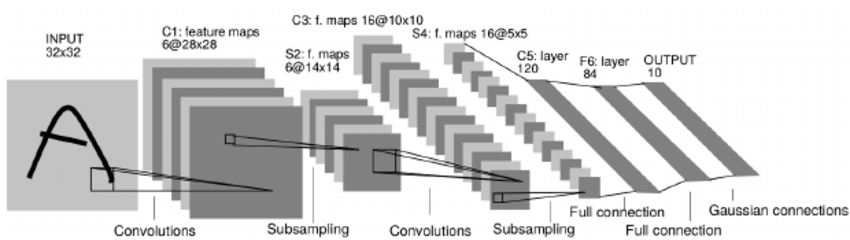
\includegraphics[width=\linewidth]{images/lenet5.png} \caption{LeNet 5}
    
	The architecture of LeNet 5, a Convolutional Neural Network used for digit recognition. \cite{LeCun1998Gradient-basedRecognition}

	\label{fig:lenet}
\end{figure}

\subsection{CNN Architecture}
A typical CNN has three types of layers:

\begin{itemize}
	\item 
Convolutional Layer
	\item 
Pooling Layer
	\item 
Fully Connected Layer
\end{itemize}

A convolutional neuron is connected with just a few neurons from the previous layer. Because of this limited connectivity, a convolutional layer focuses on a particular patch of the input. The capacity of a CNN can be controlled by varying depth and breath. CNNs work well on images since they make good premises about the characteristics of images such as local pixel dependencies and stationarity of statistics. \cite{KrizhevskyImageNetNetworks}

The kernel describes the set of weights learnt from that particular patch. The other neurons, that also share the same kernel, focus on the other areas of the input. It can be seen as a filter that is sliding through the input and each sliding window produces a set of outputs.

% FIGURE: kernel
\begin{figure}[H]	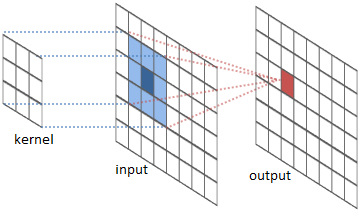
\includegraphics[width=0.5\linewidth]{images/kernel_convolution.png} 
    \centering

	\caption{The weights and the window are described by the convolution kernel.}

	\label{fig:kernel}
\end{figure}

\subsection{CNN Parameters}